\chapter{模型简介}
\label{chap:machine-learning-models}

同一批已标注邮件，可以支持几种不同的预测办法：学习特征权重，逐层执行条件规则，或者保存旧邮件、在预测时查找相近记录。第\ref{chap:introduction}章只选择了第一种形式，并用训练确定其中的参数。三种办法可能给新邮件贴上相同的标签，内部保存的东西却很不一样：一个只保留固定权重，一个保留分支条件，一个依靠历史实例；有的直接计算得分，有的还描述类别概率。只看最终标签，我们无法说出它们差在哪里，也无法判断数据变多、任务改变或需要风险判断时哪一种更合适。本章要回答：比较这些模型时，应该考察哪些对象？

回答这个问题，需要逐一追问一个模型在预测前后做了什么。它要保存多少信息，这些信息会不会随数据增加？它是直接算出一个结果，还是描述结果的不确定性？输入和输出之间按什么形状联系？它交给使用者的是什么？训练时又凭什么在候选模型之间作选择？这五个问题分别对应本章的五个维度：表示规模、概率语义、关系形式、输出接口和学习目标。前四项描述模型本身；最后一项把任务评价接到模型选择上，属于完整的学习设定，而不是预测函数的属性。讨论这五项之前，先要分清模型族、具体模型和训练三个层面，否则“模型保存了什么”和“训练怎样得到它”容易混在一起；最后再把分类和聚类放进同一组维度中比较，检查这套描述能否区分章首的三种办法。

\section{什么是模型}
\label{sec:models-meaning}

“模型”一词在日常使用中既可以指“逻辑回归”这样一类方法，也可以指训练结束后那组具体权重。比较模型之前，先要把这两种用法分开。

在第\ref{chap:introduction}章的邮件例子中，预测输入仍是$\bm{x}=(x_1,x_2)^{\top}$，两个分量分别表示促销词次数和链接数。规定“加权求和后计算垃圾邮件概率”，只确定了一种计算形式，还没有确定权重。权重不同，同一封邮件得到的概率也可能不同，因此训练前我们面对的是一组候选关系，训练后才从中选出实际使用的一项。第\ref{chap:introduction}章把满足给定形式与约束的候选集合称为\term{候选模型类}，记为$\mathcal{H}$：它列出训练允许选择的全部关系。其中的$h\in\mathcal{H}$称为候选模型，训练选出的具体成员称为训练模型。这个集合也常称模型族（model family），统计学习文献又称假设空间。聚类、降维与分布建模同样需要规定候选对象，只是对象不一定是预测函数，也可能是一组中心、一个投影或一个分布。

候选范围确定之后，还要填入使模型可以实际计算的信息：邮件分类要确定特征权重，聚类可能要确定中心位置，数据压缩可能要确定投影方向。这些量的对象不同，作用却相同，都把模型族中的一种可能形式落实为一个具体模型。第\ref{chap:introduction}章把这类在选定表示下由数据估计、用来确定具体模型的量称为模型参数；回归系数、中心坐标和网络权重都属于此类。我们用$\bm{\theta}$记录它们，$h_{\bm{\theta}}$表示参数取$\bm{\theta}$时的具体模型。

为了把“一个函数”和“一组候选函数”并排写出，我们沿用邮件参数$\bm{\theta}=(b,w_1,w_2)^{\top}$，写成
\begin{equation}
  \begin{aligned}
    h_{\bm{\theta}}(\bm{x})
      &=\frac{1}{1+\exp[-(b+w_1x_1+w_2x_2)]},\\
    \mathcal{H}&=\{h_{\bm{\theta}}:\bm{\theta}\in\mathbb{R}^{3}\}.
  \end{aligned}
  \label{eq:models-family-example}
\end{equation}
其中，$w_1,w_2$是两个特征的权重，$b$是在加权和之外加入的偏置。
集合$\mathcal{H}$包含所有允许的权重组合所确定的模型；例如，令
$b=-2$、$w_1=0.8$、$w_2=0.3$，就选出了其中一个具体模型。
这些数值是概念示例。只换参数，仍是在同一集合内选择；换成条件分支树，则改变了候选关系的形式，属于另一模型族。

候选模型类只说明可以选什么，还没有说明怎样选。对需要拟合参数的设定，学习规则利用训练样本构造学习目标，并规定初始化、参数更新、何时停止以及最终取出哪组参数；邮件例子的梯度下降就是其中的求解算法。近邻等实例方法不必求解参数拟合目标，但仍须规定保留哪些记录、新输入怎样检索邻居、怎样汇总邻居的答案。即使候选范围不变，换一种优化步骤也可能选出不同的训练模型。三个层面于是各有分工：候选模型类说明允许选什么，学习规则说明怎样从训练样本作出选择，训练模型是实际选出的结果。

网络有几层、聚类设几簇、查询参考几个邻居，也会影响这一过程。这些超参数或者划定模型族（固定网络结构后才知道有哪些连接权重），或者约束学习规则（固定邻居数后才知道每次投票使用几个实例），可以预先约定，也可以用验证样本选择。需要注意，配置项少不等于预测只需保留少量信息：近邻方法只有一个邻居数，却要依赖全部保存的样本。下一节专门讨论这个区别。

邮件数据也可以用于分组、压缩或描述特征分布。分组可保存代表中心，压缩可保存低维子空间，分布建模则说明特征怎样共同出现，输出相应地从类别变为组号、坐标或分布。无论任务怎样变，比较时都要追踪同样几件事：模型用什么表示规律，怎样据此处理输入，表示中的未知量从哪里获得，结果以什么形式交出。

表\ref{tab:models-dimensions}把这些问题整理为五个维度。它们可以同时描述一个模型，因而不是一组互斥类别；某一项也不能直接推出其余各项，例如知道一个模型是非线性的，并不能由此知道它是否建立概率分布。

\begin{table}[htbp]
  \centering
  \small
  \begin{tabularx}{\linewidth}{@{}lXX@{}}
    \toprule
    \textbf{维度} & \textbf{要回答的问题} & \textbf{主要观察方向} \\
    \midrule
参数化方式 & 模型表示规模是否有固定上限？ & 参数化、非参数化及半参数化组合 \\
    概率语义 & 是否为有关变量明确建立概率分布？ & 非概率、概率 \\
    关系形式 & 有关变量怎样发生联系？ & 线性、非线性 \\
    输出接口 & 使用模型时返回什么？ & 组织形式与结果含义 \\
    学习目标 & 怎样评价候选模型？ & 逐样本差异、关系与结构、轨迹与长期目标 \\
    \bottomrule
  \end{tabularx}
  \caption{认识模型的五个维度。每个维度回答不同问题，不能由其中一项直接推断其余各项。}
  \label{tab:models-dimensions}
\end{table}

以式\eqref{eq:models-family-example}为例，五个维度上的回答依次是：逻辑回归保存三个参数，用概率描述类别，以线性得分联系输入，返回类别概率，按概率与标签的吻合程度选择参数。如果只记录最后的垃圾邮件标签，这些选择都不可见。下面先考察预测时必须保留的信息及其规模，再逐项讨论其余维度，例子也扩展到分组和压缩。

\section{参数化方式}
\label{sec:models-capacity}

假设训练邮件由一百封增为一万封。线性分类器可以继续保存原有的三个数，只是数值更准；近邻方法则可能保存更多邮件，树模型也可能增加分支。数据增多后模型能不能、以什么方式容纳更多信息，直接影响它能表达多细的关系。候选模型能表达的关系有多丰富，称为\term{容量}（capacity）。考察表示规模怎样随数据变化，是理解容量的一个直观入口。

这一节要判断的对象始终是整个模型族，而不是某次训练得到的具体结果：某次训练恰好只用了有限个量，不能证明所有候选都受同一上限约束。参数个数也不是完整的容量度量，参数的取值范围和结构同样限制能表达的关系；这些限制怎样影响泛化，将由第\ref{part:learning-theory}部分分析。

\subsection{参数化模型}
\label{sec:models-parametric}

邮件例子中的逻辑回归代表了最简单的情形：不管训练邮件有多少，预测时只需要那三个数。输入表示和配置选定后，若模型族中的每个候选都由预先固定维数的参数向量描述，就称为\term{参数化模型族}（parametric model family），简称参数化模型。白话地说，这类模型先选定形式，再用数据填入其中固定数目的未知量。记参数维数为$p$，候选参数限制在$\mathbb{R}^{p}$的某个范围内；训练样本的记录数$n$增加可以改变参数的取值，却不会自动增加$p$。

线性回归给出了最直接的例子：$d$维输入需要$d$个权重和一个偏置，参数维数为$p=d+1$，无论用一百还是一万个样本估计，最终预测都只需这$d+1$个数。固定层数、宽度和连接方式的神经网络也一样：参数可能多达数百万个，但数量由结构配置规定，不因样本数增加而自动增长。

同样的判断也适用于分组和压缩。\term{K均值模型}（K-means）用$k$个中心代表$k$个群组：训练时交替地把每个样本分给最近的中心、再把每个中心移到所分样本的均值处，预测时把新样本分给最近的中心。固定输入维数$d$和中心数$k$后，它只需学习并保存$kd$个坐标。\term{主成分分析}（principal component analysis, PCA）寻找数据变化最大的几个方向，把样本投影到这些方向上，用少量坐标近似原样本；它保存均值和投影方向，固定原始维数和保留方向数后，表示规模也是固定的。新记录可以移动中心或方向，却不要求为每条记录再增加一套参数。

\subsection{非参数化模型}
\label{sec:models-nonparametric}

\paragraph{非参数化模型的定义}

固定维数带来一个限制：如果选定的形式与真实关系差得较远，数据再多也只能在这个形式内部调整。另一种选择是让数据增加时模型也能补充表示，从而保留更细的局部关系。\term{非参数化模型族}（nonparametric model family）允许候选关系超出预先固定的有限维参数形式，也就是说，表示规模可以随数据增长。这个名称放宽的只是固定维数限制，并不意味着模型中没有需要确定的数值，也不意味着没有需要选择的配置。

因此，判断一个模型是否属于非参数化，不看它有没有名为“参数”的量，而看给出预测所需的表示规模会不会随样本数$n$增长。具体分两步：先把输入表示、超参数和结构配置全部固定，再检查预测规则必须依赖多少随数据确定的量。只数配置的个数，会在下面的例子上得出错误结论。

我们可以直接保存邮件及其标签，每次对新邮件查找最近的$k$封，再按它们的标签投票。这就是\term[k近邻]{$k$近邻}（$k$-nearest neighbors, $k$NN）的分类规则。$k$是每次查询参考多少邻居的配置，但固定$k=3$并不能单独给出预测，还需要知道各实例的位置和标签：用一百个样本时保存一百组特征与标签，用一万个时保存一万组；哪三个邻居参与投票，由新邮件与全部实例的距离决定。所以kNN虽然只有一个配置$k$，仍属于非参数化模型；决定其表示规模的是保存的实例数，而不是$k$。

这里容易把两个$k$混为一谈。K-means的$k$是中心数量：$k$固定后，模型保存的中心坐标就固定为$kd$个。kNN的$k$只是每次查询使用的实例数：$k$固定后，保存的实例总数仍随数据增加。图\ref{fig:models-neighbors-prototypes}把实例、查询点与中心分别画出，可以对照两项限制各自约束的对象。

\begin{figure}[htbp]
  \centering
  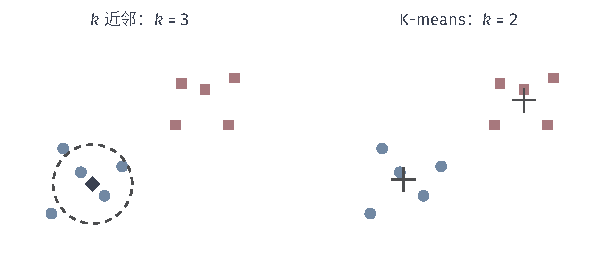
\includegraphics[width=101.406mm]{figures/06-foundations/01-basics/tikz/models-neighbors-prototypes/figure.pdf}
  \caption{两个$k$控制不同的对象。左侧kNN保存十个带标签样本，菱形表示新的预测输入，
  虚线圈内的三个近邻参加投票；右侧K-means用两个中心表示群组。
  固定近邻数不会固定实例总数，固定簇数则固定了中心数量。图为表示方式的教学示意。}
  \label{fig:models-neighbors-prototypes}
\end{figure}

\paragraph{非参数化模型的典型方法}

非参数化模型可以按表示随数据增长的方式分为几类。第一类直接保存实例。除kNN外，\term{核回归}（kernel regression）也属于这一类：预测一套新房的价格时，它按新房与各条已知成交记录的距离给这些记录分配权重，越近的记录权重越大，再对成交价取加权平均。控制“多近才算近”的带宽是配置，样本位置和成交价却随数据补充；即使带宽不变，新增一条附近的成交记录也可能改变预测。

第二类用数据确定输入空间的分区。\term{决策树}（decision tree）逐层比较特征与阈值，例如先问促销词是否达到某个次数、再问链接数，把输入分到一个区域，再给出该区域的预测。不设叶数上限时，更多数据可以支持更细的分支，阈值和叶输出的数量都能增长。\term{随机森林}（random forest）把多棵有差异的树的预测合在一起；只固定树的棵数还不足以限定表示规模，各树叶数可以增长时仍属于非参数化设定。反过来，同一类模型加上固定上限后可能转为参数化：决策树若固定深度或叶数上限，表示规模就被固定下来。第三类把预测写成训练样本贡献的加权和，使用高斯核的支持向量机就是一例，下一小节会借它澄清一个常见误解。

这些方法换来灵活性，也带来自己的假设。以kNN为例，距离与特征尺度决定谁是邻居：把链接数的单位放大十倍，邻居就可能换一批；$k$决定参考范围；实例越多，存储和查询成本越高。判断规模时还要看预测关系实际依赖什么，而不是程序保存了多少文件：线性回归程序也可能为了重新训练或来源追踪保留全部数据，但它的预测函数仍只需要固定权重。

\paragraph{与参数化模型的对比}

两类模型的差别落在两点：形式是否预先固定，表示规模是否随数据扩展。参数化模型只保存固定数目的量，预测通常更快、存储更少，样本有限时也能估计；代价是一旦固定形式与真实关系偏差较大，再增加数据也只能在这个形式内逼近，留下系统性偏差。

非参数化设定允许表示随样本扩展，具体代价则取决于所选方法。以近邻和局部平滑为例，它们依赖“附近有足够多的样本”。输入维数升高时，要让局部邻域里仍有样本，所需样本数会急剧增加；同时，高维空间中各点之间的距离往往相差不大，“最近”逐渐失去区分作用。这类随维数升高而出现的困难称为\term{维数灾难}（curse of dimensionality）。这些局部方法在远离已观测范围时也缺少邻近依据。不过，距离依赖和外推困难不是所有非参数化方法的定义属性；能否外推、怎样外推，还取决于趋势、核与其他结构假设。

因此不能笼统地说哪一类更好：固定形式贴合问题且样本有限时，参数化模型更稳定高效；关系复杂、数据充足且维度可控时，非参数化模型能利用更多局部信息。近邻、树与局部平滑的系统比较可参见统计学习教材\scite{hastie2009}。

\subsection{半参数化模型}
\label{sec:models-semiparametric}

\paragraph{半参数化模型的定义}

前两类选择是整体的：要么全部采用固定形式，要么全部让数据决定。实际问题中，我们常常对一部分关系有把握，对另一部分没有。例如房价预测中，面积的作用近似为固定增量，可以用一个线性系数表示；楼龄与房价的关系却可能先降后升，不便预先规定曲线形式。若整体用线性模型，楼龄部分会出现系统偏差；若整体用非参数化模型，又浪费了“面积作用近似线性”这一可靠知识。\term{半参数化模型}（semiparametric model）把这两种处理放进同一个模型：一部分用固定有限维参数表示，另一部分用随数据扩展的非参数化方式表示。记面积为$x$、楼龄为$z$，一个教学设定是
\begin{equation}
  f_{\beta,g}(x,z)=\beta x+g(z).
  \label{eq:models-semiparametric}
\end{equation}
系数$\beta$描述面积的固定线性作用，未知函数$g$描述楼龄与房价之间的关系，可以用局部平滑等非参数化方法估计；学习时既要确定$\beta$，也要估计整条函数$g$。判断半参数化的标准是模型中同时存在固定有限维部分与随数据扩展的部分。“参数个数居于两种方法之间”或“只有一部分参数已知”，都不是这里的含义。

一个常见误解是：模型只用了部分训练样本，规模就介于两类之间，因而是半参数化。支持向量机的几种设定可以说明这个判断为什么不成立。\term{支持向量机}（support vector machine, SVM）先计算一个实数得分$s(\bm{x})$，再按得分正负分类；它在训练时还要求样本不仅落在边界正确一侧，而且离边界留出余量。硬间隔版本把这一要求写成必须满足的约束，软间隔版本则允许部分样本违反，但在学习目标中惩罚错分或余量不足。余量的几何意义留到第\ref{sec:models-spatial-objectives}节，这里只看它采用哪一种表示。

固定$d$维输入的线性SVM使用$s(\bm{x})=\bm{w}^{\top}\bm{x}+b$，预测只需$d$个权重和一个偏置，是固定维数的表示。线性得分只能给出平面或超平面边界。若想得到弯曲边界，可以先把输入映射为一组新特征$\bm{\phi}(\bm{x})$，再在新特征上计算线性得分；但新特征可能极多，逐一写出并不现实。核函数（kernel function）$\kappa(\bm{u},\bm{v})$绕开了这一步：它直接用原始输入算出两个样本映射后的内积，即$\kappa(\bm{u},\bm{v})=\langle\bm{\phi}(\bm{u}),\bm{\phi}(\bm{v})\rangle$，可以理解为某种意义下两个样本的相似度。SVM的最优权重可以写成训练样本映射后特征的加权组合，代入线性得分，得分便只依赖样本之间的核函数值：
\begin{equation}
  s(\bm{x})=\sum_{i\in I_{\mathrm{SV}}}
    a_i\,\kappa(\bm{x}_i,\bm{x})+b.
  \label{eq:models-support-vector-expansion}
\end{equation}
式中$a_i$为学习得到的系数，$I_{\mathrm{SV}}\subseteq\{1,\ldots,n\}$收集系数非零的训练记录索引。预测新输入$\bm{x}$时，只有这些记录通过核函数值$\kappa(\bm{x}_i,\bm{x})$参与得分，它们的预测输入向量称为\term{支持向量}（support vectors）。在软间隔SVM中，系数非零的通常是落在边界附近、余量不足或被错分的样本；离边界足够远的样本系数为零，删去它们不改变得分。

于是模型看起来只依赖部分样本。判断规模仍要回到表示本身：预测所需的量会不会随$n$增长？若$\bm{\phi}$是有限维的，式\eqref{eq:models-support-vector-expansion}中的求和可以先合并成固定维权重$\bm{w}=\sum_{i}a_i\bm{\phi}(\bm{x}_i)$，得分写成$\bm{w}^{\top}\bm{\phi}(\bm{x})+b$，模型就是参数化的；线性SVM取$\bm{\phi}(\bm{x})=\bm{x}$，属于这种情形，固定次数的多项式核也对应有限维特征。常用的高斯核$\kappa(\bm{u},\bm{v})=\exp(-\lVert\bm{u}-\bm{v}\rVert_2^2/(2h^2))$（$h>0$为带宽）则不同，它对应的特征映射是无穷维的，无法合并成固定维权重；预测只能保留支持向量及其系数，而支持向量数一般随样本增加。因此高斯核SVM通常属于非参数化模型。某次训练只保留了有限条支持向量，只是这一次的结果；固定带宽也不固定支持向量数。

真正意义上的半参数化SVM，要在预测关系中同时保留固定系数表示的线性趋势和由核模型学习的非参数化修正项，并联合估计两者\scite{smola1998semiparametric}。三种设定放在一起说明：容量不能只凭“SVM”这个名称推断，也不能只凭它使用了核或只保留部分样本，而要检查特征空间和候选表示本身。

\paragraph{与参数化、非参数化模型的对比}

半参数化模型的收益来自分工：参数化部分保留可解释、易估计的主要关系，例如面积系数$\beta$可以直接读作每平方米的价格增量；非参数化部分承接剩余的复杂结构，避免把楼龄的影响强行压进固定曲线。代价是估计和检验更复杂：$\beta$与$g$要联合估计，两部分若相关（例如新房普遍面积更大），还要说明它们是否真的可以分开识别。因此它不是“规模居中的非参数化模型”，而是两类部分各自承担明确职责的组合。

\section{变量的概率语义}
\label{sec:models-probability}

表示规模说明模型保存多少信息，却没有说明它怎样对待结果的不确定性。以明日温度为例，即使气象观测完全相同，实际温度也会有起伏。模型可以直接预测$22\,^{\circ}\mathrm{C}$，也可以描述温度落在各范围的概率，例如大概率落在$20$至$24\,^{\circ}\mathrm{C}$之间。判断属于哪一种，依据是模型内部有没有为有关变量建立分布，而不是最终交付点值还是完整分布：建立了分布的模型也可以只返回均值。这个区别同样适用于分类、分组与压缩。

\subsection{非概率模型}
\label{sec:models-nonprobabilistic}

模型用函数、规则或几何关系直接取得结果，不为当前变量明确建立分布，就称为\term{非概率模型}（non-probabilistic model）。在温度预测中，记气象特征为$\bm{x}$、模型参数为$\bm{\theta}$，模型计算
\begin{equation}
  \hat{y}=f_{\bm{\theta}}(\bm{x}).
  \label{eq:models-point-prediction}
\end{equation}
训练时根据预测温度与实际温度的偏差调整参数；使用时把新的观测代入函数，得到一个预测值，例如$22\,^{\circ}\mathrm{C}$。这个点值没有给出偏离程度的概率，更高或更低温度的可能性需要另外说明。

同一类直接计算还出现在分组和压缩中：K-means找中心、让样本靠近所属中心，预测时返回最近中心编号；PCA找投影方向，用少量坐标保留主要变化。中心距离和投影已经规定了计算，不需要先为样本假定概率分布。温度偏差、簇内距离或重构误差都可以直接服务于点预测、分组或压缩；但“温度偏离预测超过两度的概率是多少”这类问题，这些输出回答不了，需要额外建立概率关系。

\subsection{概率模型}
\label{sec:models-probabilistic}

要回答“偏离超过两度的概率”这类问题，就要把温度视为随机变量，给各个取值范围赋概率。\term{概率模型}（probabilistic model）为任务涉及的随机变量及其关系建立概率分布，也就是说，它不只给出一个答案，而是描述各种可能答案各有多大可能。对于温度预测，最简单的做法是保留原来的预测函数，让它给出分布的中心，再用方差描述围绕中心的起伏：
\begin{equation}
  y\mid\bm{x}\sim\mathcal{N}\bigl(\mu_{\bm{\theta}}(\bm{x}),\sigma^2\bigr).
  \label{eq:models-linear-gaussian}
\end{equation}
这里$y\mid\bm{x}$表示给定气象特征$\bm{x}$后的温度，$\mu_{\bm{\theta}}(\bm{x})$给出该条件下的均值；$\bm{\theta}$是均值函数的参数，$\sigma^2>0$是另一个需要从数据中估计的模型参数，完整参数由二者组成。$\mathcal{N}(\mu,\sigma^2)$表示均值为$\mu$、方差为$\sigma^2$的高斯分布。在均值$22\,^{\circ}\mathrm{C}$、标准差$2\,^{\circ}\mathrm{C}$的教学设定中，均值给出与点预测相同的中心值；分布额外说明偏离中心的温度有多大可能，例如落在$20$至$24\,^{\circ}\mathrm{C}$（均值左右各一个标准差）的概率约为$68\%$。图\ref{fig:models-point-distribution}对照了这两种预测形式。

\begin{figure*}[htbp]
  \centering
  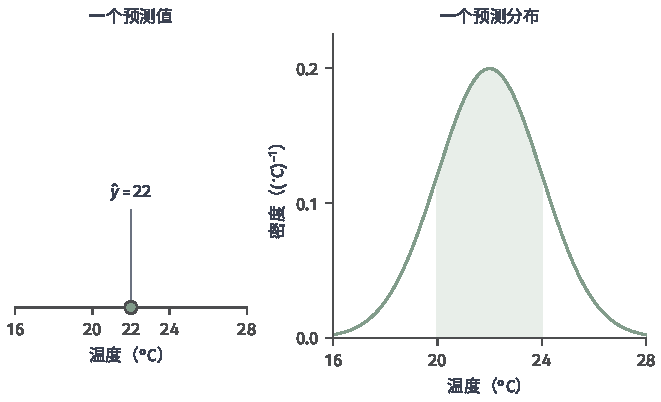
\includegraphics[width=112.000mm]{figures/06-foundations/01-basics/matplotlib/models-point-distribution/figure.pdf}
  \caption{同一温度预测的两种描述。左侧只给出一个预测值；右侧给出高斯预测分布，
  阴影面积表示温度落在$20$到$24\,^{\circ}\mathrm{C}$之间的概率。数值用于教学示意。}
  \label{fig:models-point-distribution}
\end{figure*}

分组和降维也有成对的非概率与概率做法。K-means保存中心并比较距离。\term{高斯混合模型}（Gaussian mixture model, GMM）则假设每个样本先按一定比例随机属于某一组，再从该组的高斯分布中产生；每组因此有中心、分散程度和总体比例三类参数。处于两组之间的样本，K-means按最近中心给出唯一组号，GMM则可以计算它属于各组的后验概率，组的大小、形状与重叠都参与判断。PCA通过线性投影压缩与重构；\term{概率主成分分析}（probabilistic PCA, PPCA）在低维线性表示上加入高斯分布和观测噪声，说明观测怎样分布在子空间附近，并能估计缺失观测的分布\scite{tipping1999}。

\paragraph{判别式与生成式建模}

回到邮件分类。给定邮件特征后，我们要的是类别概率$p(y\mid\bm{x})$。得到它有两条路线，区别在于模型描述哪个分布。

第一条路线直接描述我们要的条件概率，称为\term{判别式建模}（discriminative modeling）：模型只学习“看到这些特征时各类别有多大可能”，不关心特征本身怎样产生。逻辑回归就是这样做的，它用带标签样本调整权重，使类别概率与观测标签吻合，无须描述输入特征的总体分布或每一类内部的特征分布。更广义的判别式路线还包括只学习分类得分或类别预测规则的SVM；这里固定概率输出，以便与另一条路线比较。

第二条路线绕一步：先描述每一类邮件“长什么样”，再反推类别，称为\term{生成式建模}（generative modeling）。它规定每类有多常见、每类内部的输入如何分布，由此建立联合分布$p(\bm{x},y)=p(y)p(\bm{x}\mid y)$：$p(y)$描述各类别的比例，$p(\bm{x}\mid y)$描述每一类内部的特征分布。有了这两部分，再对新输入用贝叶斯公式反推类别。对于编号为$1,\ldots,k$的类别，
\begin{equation}
  p(y=c\mid\bm{x})
  =\frac{p(y=c)\,p(\bm{x}\mid y=c)}
         {\sum_{j=1}^{k}p(y=j)\,p(\bm{x}\mid y=j)}.
  \label{eq:models-generative-classification}
\end{equation}
分子是$c$类的比例与该类产生输入$\bm{x}$的可能性之积，分母对所有$k$类的这一乘积求和，使各类结果之和为一；所得称为类别后验概率，“后验”指看到输入之后对类别的判断。式子要求分母大于零，即至少有一类可能产生$\bm{x}$。若只需输出概率最大的类别，比较各类分子即可，因为分母对所有类别相同。例如，构造两类邮件比例$p(y=1)=0.2$、$p(y=0)=0.8$，标签$1$表示垃圾邮件；某组计数$\bm{x}$在两类内部的概率分别为$0.12$与$0.01$，类别比例乘以类内概率得到$0.024$与$0.008$，归一化后垃圾邮件概率为$0.024/(0.024+0.008)=0.75$。

生成式路线的难点在类内分布$p(\bm{x}\mid y)$：特征一多，各特征的联合分布很难直接估计。\term{朴素贝叶斯}（naive Bayes）用一个简化假设处理这个难点：给定类别后各特征相互独立，于是$p(\bm{x}\mid y)=\prod_{j}p(x_j\mid y)$，只需逐个估计单个特征的类内分布（条件独立的定义可参考\BookVolumeRef{vol:mathematical-preliminaries-lower}{卷2《数学准备：概率、因果与决策》}）。这个假设常常不精确，例如促销词多的邮件往往链接也多。\term{高斯判别分析}（Gaussian discriminant analysis）同样从类内分布出发，但采用多元高斯，能保留特征之间的相关性。“生成式”描述的是分布假设的方向：先按$p(y)$取得类别，再按$p(\bm{x}\mid y)$取得特征。在邮件案例中，这些特征只是计数，能够生成计数并不等于能够生成完整正文，后者需要文本分布。

两条路线描述的对象不同，训练时评价的概率也不同。对独立同分布的带标签样本，判别式使用条件负对数似然，累加$-\log p_{\bm{\theta}}(y_i\mid\bm{x}_i)$；生成式使用联合负对数似然，累加$-\log p_{\bm{\theta}}(\bm{x}_i,y_i)$。即使最后的类别后验形式相同，拟合不同的概率对象仍可能得到不同参数：判别式把全部数据用于类别关系，生成式还要拟合特征分布，描述范围更广，假设成立时还能采样或补全缺失特征，但也要估计更多关系\scite{ng2001}。图\ref{fig:models-discriminative-generative}把相同的类别后验放到两条路线中：判别式直接学习后验，生成式先学习联合分布再计算后验。下方两个面板应分开读：左面板的条件类别概率在每个输入处总和为一，右面板的联合密度同时包含特征分布与类别比例，二者的数值代表不同对象。

\begin{figure*}[!htb]
  \centering
  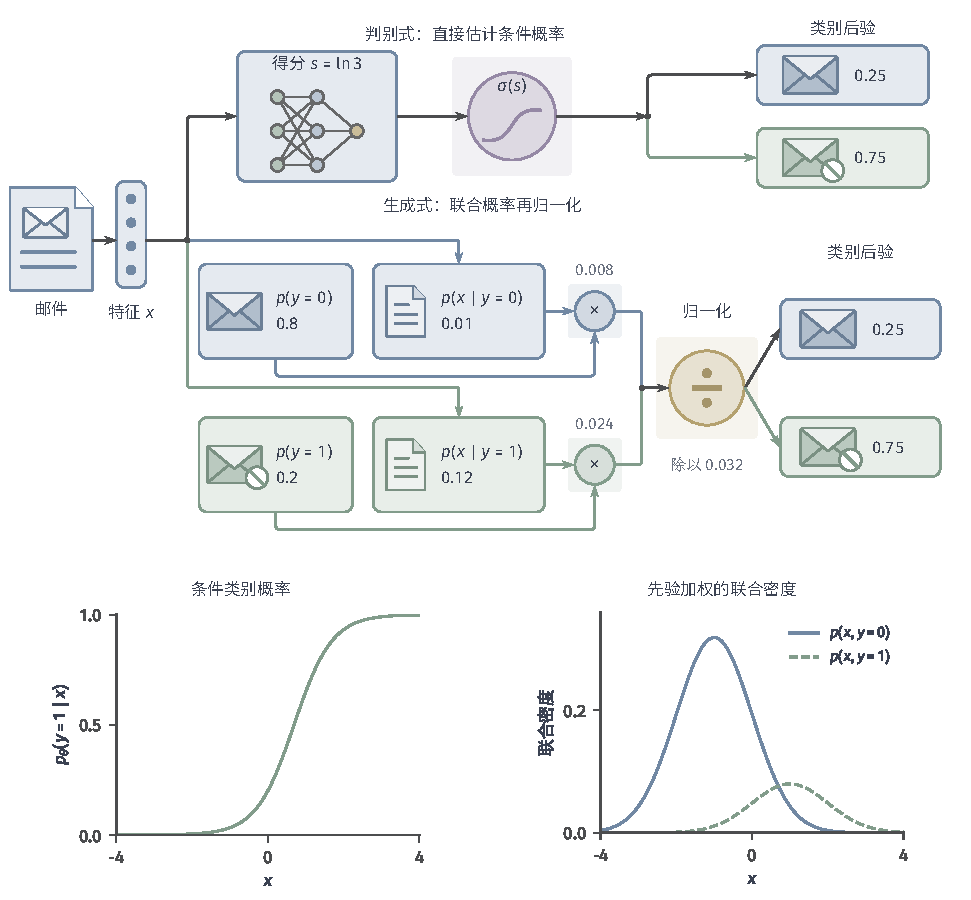
\includegraphics[width=164.600mm]{figures/06-foundations/01-basics/tikz/models-discriminative-generative/figure.pdf}
  \caption{两条分类建模路线。上部框图中的判别式路线以二分类Logistic读出为例，令得分$s=\ln3$，则$\sigma(s)=0.75$，得到类别后验$p(y=1\mid x)=0.75$、$p(y=0\mid x)=0.25$。生成式路线沿用离散邮件教学数值，先验$0.8$、$0.2$与类内事件概率$0.01$、$0.12$相乘，分别得到联合概率$0.008$、$0.024$，再除以总和$0.032$。两条路线的数值仅作可核算示意，不假定实际训练结果相同。下方两个面板另用连续构造：先验$0.8$、$0.2$分别对应$\mathcal{N}(-1,1)$、$\mathcal{N}(1,1)$。左面板为条件类别概率，右面板为先验加权的联合密度，整个实数轴上的两条密度曲线面积分别为$0.8$与$0.2$；这些密度值不与上部离散事件概率对应。}
  \label{fig:models-discriminative-generative}
\end{figure*}

\paragraph{概率模型的推断}

建立分布之后，概率模型要处理两类计算：参数已知时用模型回答问题，参数未知时用数据确定参数。前一类称为\term{概率推断}（probabilistic inference）：利用模型分布和已观测的信息计算所需概率，例如式\eqref{eq:models-generative-classification}由类别比例和类内分布算出类别后验，高斯温度模型算出温度落在某区间的概率。固定训练所得模型、对新输入计算这些结果，就是预测。变量很多、依赖复杂时，这些条件分布的计算本身就是难题，属于\term{概率图模型}（probabilistic graphical model）专题，可参考\BookVolumeRef{vol:probabilistic-graphical-models}{卷6《模型：概率图模型》}。还要注意，推断给出的是“在这个模型下”的概率；这些概率与实际频率是否相符，要另行检验，由第~\ref{chap:trust-reliability}章讨论。

\paragraph{概率模型的学习}

参数未知时，还要用训练样本确定模型本身。一个自然的想法是：好的参数应当让已经观测到的数据显得“可能”。\term{似然}（likelihood）把这一想法写成函数：固定训练样本$\mathcal{D}$，把模型赋予这些数据的概率或密度看作参数$\bm{\theta}$的函数。在最大值能够取到时，\term{最大似然估计}（maximum likelihood estimation）选择使似然最大的参数。这样选出一个参数值$\hat{\bm{\theta}}$的做法属于\term{点估计}（point estimation），预测时直接把它代入模型，得到插件预测$p(y\mid\bm{x},\hat{\bm{\theta}})$。

点估计把参数当作已经确定，不表达“参数本身也估不准”。\term{贝叶斯推断}（Bayesian inference）改为用分布描述对参数的认识：先为$\bm{\theta}$指定\term{先验分布}（prior distribution），表示看到数据前认为哪些参数值较可能；再用训练样本把它更新为参数的\term{后验分布}（posterior distribution）。注意这里的后验对象已从前文的类别$y$变成参数$\bm{\theta}$。预测时不再只用一个参数，而是让每个参数值各自给出预测分布，再按后验概率加权平均。

把这个加权平均写成公式需要两个条件。记$\Theta$为参数的允许范围，先考虑参数后验具有密度$p(\bm{\theta}\mid\mathcal{D})$（相对于Lebesgue测度）的情形。第一，给定新输入$\bm{x}$和参数$\bm{\theta}$后，新结果$y$与训练样本$\mathcal{D}$条件独立，即参数已经概括了训练数据对新结果的全部影响。第二，权重本应是同时看到$\mathcal{D}$和$\bm{x}$之后的参数后验$p(\bm\theta\mid\bm{x},\mathcal D)$；只有新输入不再提供关于参数的额外信息时，才能换成$p(\bm\theta\mid\mathcal D)$。这一条件在两种常见设定下成立：$\bm{x}$是预先固定的设计输入，或在随机输入设定下$\bm\theta$与$\bm{x}$给定$\mathcal D$条件独立。在这两个条件下，后验预测写为
\[
  p(y\mid\bm{x},\mathcal{D})
  =\int_{\Theta} p(y\mid\bm{x},\bm{\theta})
    p(\bm{\theta}\mid\mathcal{D})\,\mathrm d\bm{\theta}.
\]
被积函数的前一项是参数取$\bm{\theta}$时的预测分布，后一项是该参数的后验权重。离散参数把积分换成对允许取值的求和，更一般的后验则按其概率测度积分。与插件预测相比，后验预测把参数的不确定性也带进了预测：数据少、后验较分散时，不同参数的预测差别较大，平均后的预测分布通常更宽。学习概率模型也不改变表示规模这一维度：成分数固定的GMM可以用固定维数参数描述，是参数化概率模型；高斯过程描述一组可能函数上的概率关系，通常属于非参数化概率模型\scite{rasmussen2006}。

\paragraph{与非概率模型的对比}

概率模型的优势，来自它保留了所建模型下各可能结果的概率信息，而不只报告一个中心值。两个模型可以给出相同的中心值$22\,^{\circ}\mathrm{C}$，一个集中在$21$至$23\,^{\circ}\mathrm{C}$，另一个允许更宽的变化。若某项作业只允许温度处于$20$至$24\,^{\circ}\mathrm{C}$，我们要比较的是两个模型赋予区间外温度的概率，相同的均值回答不了这个风险问题；分布较宽也只有结合越界事件及其代价，才转化为明确的后果。同样的信息还有其他用途：GMM给交界处样本返回各组后验，而非强制编号；生成式模型可以采样或补全缺失观测；决策时可以直接把区间概率与行动代价结合。不过，这些概率是否覆盖真实波动、参数误差和模型失配，仍取决于建模、估计与检验，不能由概率接口本身保证。

代价有三方面。第一，必须假定分布形式。假设错误时，例如同类条件下温度实际有两个峰而模型用单个高斯，区间和尾部概率可能系统性失准，均值却未必错误：对称双峰分布的中心仍可能被正确估计。第二，通常要估计更多量（类别比例、类内分布、方差等），对数据量和估计质量的要求更高，生成式模型尤其如此。第三，训练之后还有计算与检验成本：复杂模型的后验和边缘概率往往没有闭式解，需要近似推断；概率输出是否与实际频率相符，必须通过校准和覆盖率检验。名义上$90\%$的区间若实际只覆盖$80\%$，按名义覆盖率安排行动的使用者就会低估越界风险；至于这比不报告概率的方案损害更大还是更小，要固定两种方案的行动规则与错误代价再比较。

因此，当任务只需要一个准确的点结果、数据有限或分布假设难以检验时，直接的非概率模型往往更简单稳定；当决策依赖风险、置信度或多种可能结果时，建立概率分布才值得这些额外成本。

\section{变量的关系形式}
\label{sec:models-structure}

确定了保存多少信息、是否建立分布之后，还要决定输入怎样变成输出。温度可能随某个特征按固定幅度变化，也可能在不同范围按不同规律变化；模型的关系形式描述的就是这项选择。本节判断一个关系是线性还是非线性，并比较实现非线性的几种方式。

“线性”的判断有三个容易混淆的前提，需要先说清。第一，要固定考察的对象：回归看预测函数，分类看得分或边界，降维看坐标映射；同一个模型可能在一个量上线性、在另一个量上非线性，后面的逻辑回归就是例子。第二，要固定以哪个输入为基准：先把$x$变成$x^2$、再计算$wx^2+b$，对新特征$x^2$是线性的，对原始$x$却不是；本章一律以原始输入为基准。第三，参数以什么方式进入模型（对参数线性）是另一个问题，上例对参数$w,b$是线性的，却不能据此说预测对输入线性。

\subsection{线性结构}
\label{sec:models-linear}

线性关系的基本特征是固定增量：先固定其他特征，一个特征每增加一单位都带来相同的预测变化。线性回归用权重记录这种增量，将$d$维输入$\bm{x}$与$\bm{w}\in\mathbb{R}^{d}$加权相加，再加偏置$b$：
\begin{equation}
  \hat{y}=\bm{w}^{\top}\bm{x}+b
  =\sum_{j=1}^{d}w_jx_j+b.
  \label{eq:models-linear-score}
\end{equation}
固定其他特征后，$x_j$每增加一个单位，预测值都改变$w_j$。例如用面积预测房价时，线性关系假设每增加一平方米带来的预测增量相同。严格说，带常数项$b$的关系称为仿射关系；机器学习中通常也将它归入线性模型。

\paragraph{分类中的线性}

分类时情况稍复杂。线性得分可以取任意实数，概率却必须在零与一之间，所以逻辑回归要先用逻辑函数转换得分。那么它还算不算线性模型？答案取决于考察哪个量。记二分类正类概率为$p$，计算及其等价变形为
\begin{equation}
  p=\frac{1}{1+\exp[-(\bm{w}^{\top}\bm{x}+b)]},
  \qquad
  \log\frac{p}{1-p}=\bm{w}^{\top}\bm{x}+b.
  \label{eq:models-logistic-structure}
\end{equation}
左式将任意实数得分转为零与一之间的概率。右式是左式的变形：$p/(1-p)$比较正类与负类的概率大小，再取对数，得到\term{对数几率}（log odds），它仍然是输入的仿射函数。用$p=0.5$作分类阈值时，两类概率相等、对数几率为零，边界因而满足$\bm{w}^{\top}\bm{x}+b=0$。当$\bm{w}\ne\bm{0}$时，这个方程在$d$维输入空间中给出一个超平面，邮件例子的二维情形就是一条直线；若$\bm{w}=\bm{0}$，概率不随输入变化，也就不存在这样的分界。因此把逻辑回归称为线性分类模型，指的是对数几率或分界关系是线性的，概率本身仍经过非线性转换。基础\term{感知机}（perceptron）同样计算加权得分再按正负分类，线性SVM也用线性分界面完成二分类；三者学习参数的准则各不相同，却可以共享同一种关系形式。

\paragraph{聚类和降维中的线性}

线性结构并不专属预测。PCA也使用线性关系，只是对象改为投影坐标：均值与方向固定后，每个坐标都是中心化输入的加权和；PPCA加入分布与噪声假设，仍保留低维表示到观测均值的线性关系。K-means没有预先给类别边界，但最近中心规则会把输入空间分成若干分配区域。两个区域的分界由到两个中心等距的点组成：取中心$\bm{\mu}_1$与$\bm{\mu}_2$，边界上的样本满足$\lVert\bm{x}-\bm{\mu}_1\rVert_2^2=\lVert\bm{x}-\bm{\mu}_2\rVert_2^2$。两边按$\lVert\bm{x}-\bm{\mu}\rVert_2^2=\bm{x}^{\top}\bm{x}-2\bm{\mu}^{\top}\bm{x}+\bm{\mu}^{\top}\bm{\mu}$展开，两边都含有$\bm{x}^{\top}\bm{x}$，相减后消去，得到
\begin{equation}
  2(\bm{\mu}_2-\bm{\mu}_1)^{\top}\bm{x}
  =\lVert\bm{\mu}_2\rVert_2^2-\lVert\bm{\mu}_1\rVert_2^2.
  \label{eq:models-kmeans-boundary}
\end{equation}
消去平方项后是输入的仿射方程，说明两个不同中心之间的分配边界是线性的。距离本身仍是二次函数，输出的离散编号也不能解释为输入的线性函数；后文把K-means放在线性一侧时，专指这种两两分配边界。


\subsection{非线性结构}
\label{sec:models-nonlinear}

固定增量假设未必适合当前对象：刹车距离通常不随速度按同一增量增长，剂量作用可能随区间改变，促销词的含义还可能依赖外部链接数。要表达弯曲、阈值和特征的共同作用，单个仿射关系未必充分。保持上一节的观察对象，如果预测值或得分不能写成原始输入的仿射函数，就称这一关系为非线性；二分类若需要弯曲或分段边界，也不能只用一个超平面。图\ref{fig:models-linear-nonlinear}用同一组中心与外圈样本比较：任何直线都无法完全分开两类，径向边界却可以，差别来自候选关系而不是评价样本。

\begin{figure}[!htb]
  \centering
  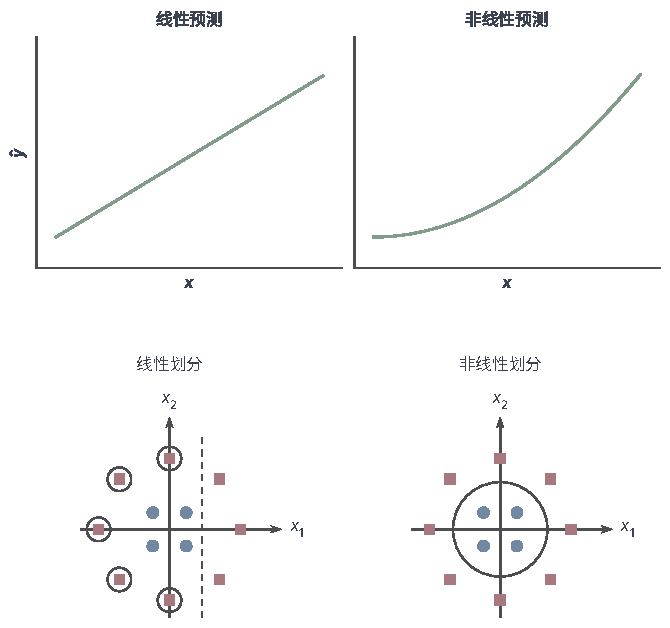
\includegraphics[width=112.000mm]{figures/06-foundations/01-basics/tikz/models-linear-nonlinear/figure.pdf}
  \caption{线性与非线性关系的几何示意。上排依次为线性预测与非线性预测，
  下排用同一组环形样本对照线性SVM的限制与二次核SVM的表达能力；圆点和方点代表两类。
  左图虚线只展示一条候选直线，空心圈标出按其左右类别分配时的错分方点，不代表最优SVM解。
  外圈方点的凸包包含内圈圆点，故任何直线都不能完全分离这组样本。
  右图以圆心为坐标原点，半径$8$的边界可由二次核
  $\kappa(\bm{u},\bm{v})=(\bm{u}^{\top}\bm{v})^2$与偏置表示。图为几何构造，非训练结果。}
  \label{fig:models-linear-nonlinear}
\end{figure}

什么时候需要离开线性关系？线性模型给出了固定增量的基线。若独立验证样本显示它在某些输入范围持续高估、在另一些范围持续低估，或误判集中于特定特征组合，就说明固定增量假设可能遗漏了弯曲、阈值或交互关系。非线性关系主要靠两种方式实现：按条件划分区域，或对输入作非线性变换。

\paragraph{按条件采用不同规则}

第一种方式先确定输入落在哪个区域，再按区域使用规则。决策树把这一步写成连续条件判断，例如促销词达到阈值后再检查链接数；根到叶的路径汇集输入要满足的条件，叶节点给出对应区域的预测。图\ref{fig:models-tree-partition}把相同条件同时画成判断树和平面区域。

\begin{figure}[htbp]
  \centering
  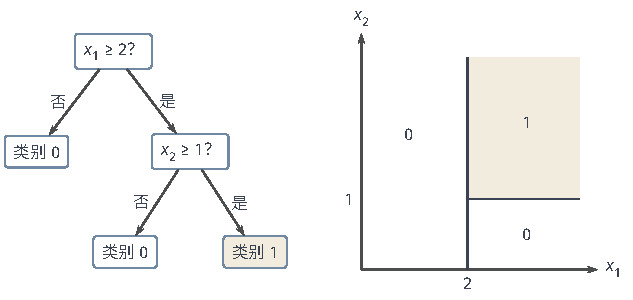
\includegraphics[width=107.209mm]{figures/06-foundations/01-basics/tikz/models-tree-partition/figure.pdf}
  \caption{按条件分情况处理输入。左侧为判断树，右侧为对应的输入区域。
  该教学例子在$x_1\geq2$且$x_2\geq1$时输出类别$1$，其余区域输出$0$。}
  \label{fig:models-tree-partition}
\end{figure}

单个特征阈值只划分两侧，多次组合却能形成复杂区域；常见树在叶节点给固定输出，跨过区域边界时预测可能跳变。这种结构适合表达条件规则，表示规模则取决于叶数：允许随数据增长是非参数化设定，固定上限则限制候选规模，所以关系形式与参数化方式仍要分开判断。

\paragraph{对输入进行非线性变换}

第二种方式先构造能表达变化的新特征，再在新特征上计算线性得分。平方项$x_1^2$可以表示弯曲，乘积$x_1x_2$可以表示交互；关系中出现$x_1x_2$时，改变$x_1$的作用会随$x_2$而变，这称为特征交互。把变换记为$\bm{\phi}(\bm{x})$，得分写为
\begin{equation}
  s(\bm{x})=\bm{w}^{\top}\bm{\phi}(\bm{x})+b.
  \label{eq:models-feature-score}
\end{equation}
变换中的非线性关系可能使这个线性得分在原空间形成非线性边界。例如中心区域是一类、外围是一类时，可以把到原点的平方距离$x_1^2+x_2^2$作为新特征，再用一个阈值区分两类。

问题在于变换从哪里来。手工加入平方项和交互项，需要预先知道哪些弯曲和交互重要。\term{核方法}（kernel methods）用第\ref{sec:models-semiparametric}小节的核函数直接计算变换后特征的内积，因而可以使用很多甚至无穷多个变换特征而不逐一写出：线性核仍对应线性关系，高斯等非线性核可以形成弯曲边界。标准高斯核SVM随样本保留更多系数，采用非参数化表示；若先固定有限个变换特征作近似，则改变了候选规模的设定\scite{cortes1995}。

神经网络进一步让中间变换也由训练确定。多层网络在相邻两次加权和之间加入\term{激活函数}（activation function），例如整流线性单元（ReLU）计算$\max\{0,u\}$，把负值置零、保留正值，使不同输入范围走不同的计算路径；训练目标同时调整这些中间表示和最终预测。激活函数不可省略：若各层都只有加权和与偏置，把第一层$\bm{W}_1\bm{x}+\bm{b}_1$代入第二层得到$\bm{W}_2\bm{W}_1\bm{x}+(\bm{W}_2\bm{b}_1+\bm{b}_2)$，仍是一个仿射函数，堆叠再多这样的层也只能表达线性关系。

树按条件改变规则，特征变换让新坐标表达弯曲与交互，两种思路可以交叉，分段线性网络也能形成不同的计算区域。无论哪一种，结构只说明能表达什么关系，并不同时规定其他维度：固定次数的多项式回归只需固定系数，是参数化的非线性模型；高斯过程同样能产生弯曲关系，却对函数建立概率分布，不受固定有限维系数限制。新样本上的效果，还要由数据、限制与训练方式支持。

\paragraph{与线性结构的对比}

非线性结构的收益是表达能力：它能刻画弯曲、阈值和交互，在真实关系确实复杂时缩小系统性偏差。代价来自学习和泛化两个环节。

学习上，候选关系变大后，目标函数可能有更多局部极小，结果对初始化和超参数更敏感，树和神经网络都需要更多调参与计算；候选规模若随数据增长，还要决定树的深度、核的带宽等配置。泛化上，表达能力越强，越容易把训练数据中的偶然波动也当作规律拟合进去。换一批训练样本，这样的模型可能变化很大，在新样本上的误差也随之升高。简单模型的误差主要来自形式不够（偏差），复杂模型则更多来自对样本的敏感（方差），二者此消彼长，常称为偏差与方差的权衡。高维稀疏数据上非线性尤其容易失效，因为每个局部区域都可能缺乏足够样本。

因此，选择非线性结构应有具体证据，例如在线性模型的残差中看到持续的结构性偏差，而不是默认“更复杂一定更好”；同时用结构限制（层数、深度、正则化）和独立验证，把表达能力约束在数据能够支撑的范围内。

\FloatBarrier
\section{输出的形式与含义}
\label{sec:models-output}

设定了模型内部的计算关系以后，还要决定把哪些结果交给使用者。温度预测可以只返回一个数，也可以提供预测区间或完整分布；邮件分类可以直接返回类别，也可以同时列出类别概率。说明输出要分两步：先说明结果按什么形状组织——标量、向量，还是保留位置与顺序的对象；再说明其中数值代表什么——预测值、类别编码、分布摘要、完整分布，还是一次采样结果。只给出形状，使用者仍不知道这些数怎样用于判断。

\subsection{输出的组织形式}
\label{sec:models-output-form}

\paragraph{标量输出}
\label{sec:models-scalar-output}

温度预测若只返回$22\,^{\circ}\mathrm{C}$，结果便由一个数及其单位构成。价格预测和商品评分也常采用这种\term{标量输出}（scalar output）。使用时，数值必须连同单位或评分尺度一起解释。

一个数也可以用作编号。邮件分类中的$0$与$1$可分别表示正常邮件和垃圾邮件，聚类中的$1,2,\ldots,k$则区分发现的群组。前者的含义由预先定义的标签确定，后者的含义来自分组结果。交换簇编号不会改变哪些样本同属一组，因而编号之差通常不能解释为距离。

\paragraph{向量与结构化输出}
\label{sec:models-vector-output}

同时预测温度、湿度和风速时，单个数已经容纳不了全部结果，我们需要按约定次序返回三个分量。这便是\term{向量输出}（vector output）。未来七天的温度也可以组成向量，不过此时分量依次对应日期。使用任何这样的结果，都要知道各坐标对应的对象、单位和顺序。

向量还可以描述输入，而不直接给出任务答案。PCA的输出坐标记录样本沿各投影方向的位置，神经网络也可以把图像映射成用于检索或分类的特征向量。同一图像经过裁剪、颜色变换等处理得到的输入版本称为\term{视图}（view）。若这些变换按任务设定保留内容含义，训练便可以要求不同视图的表示在指定距离或相似度下接近；这里需要保留的是表示之间的关系。

重构图像时，输出虽也是一组数值，却必须按像素位置和颜色通道还原成数组；文本要保留符号顺序，还可能具有不同长度。对于这些结构化结果，分量值与位置、顺序或连接关系共同决定含义，不能任意交换坐标。因此，只确定组织形式还不够：同样形状的输出，其中的数代表什么仍需单独说明。

\subsection{输出的含义}
\label{sec:models-output-semantics}

第\ref{sec:models-probability}节判断的是模型内部是否为变量建立分布；这里查看使用者实际收到什么。模型可能交付完整分布，也可能只返回由分布计算出的类别、均值或区间，因此模型内部保留的信息与接口交付的信息要分别说明。

\paragraph{点结果与分布摘要}

直接结果可以是一个预测值、类别或簇编号。即使内部建立了概率分布，接口也可以只返回摘要：逻辑回归选出概率最大的类别，高斯温度模型报告均值或预测区间。摘要使比较与决策更方便，却省略了部分可能结果及其概率。因此，输出一个点或区间，并不能据此判断模型内部有无概率语义。

\paragraph{概率分布与采样}
\label{sec:models-distribution-output}

若使用者需要比较各个结果的可能性，接口就应保留\term{概率分布输出}（probability distribution output）。有限类别可以逐项列出非负且总和为一的概率。例如，邮件分类的$(0.2,0.8)^{\top}$分别给正常邮件和垃圾邮件赋予$0.2$与$0.8$。它比单个类别标签多保留了概率如何分配的信息。不过，这些数能否对应实际频率，还要通过校准检验，不能仅凭概率集中就宣称预测可靠。

连续结果通常无法逐个列出概率，而是通过分布形式及其参数说明。例如，指定高斯分布并给出均值$22$、方差$4$，就确定了温度的密度曲线。某一区间对应的曲线下面积才是落入该区间的概率；单点的曲线高度是密度，不能当作恰好取该值的概率。

一个概率模型由此可以提供三种接口：交付分布、计算摘要，或从分布采样。温度模型可以报告均值$22\,^{\circ}\mathrm{C}$，也可以给出包含指定模型概率质量的预测区间；后者的名义概率水平是否达到实际频率覆盖，需要另用未参与训练的数据检查。一次采样则可能返回$21.3\,^{\circ}\mathrm{C}$。图像生成也遵循这个区别：分布描述可能图像，采样才产生一张具体图像，多次采样可以产生不同结果。

因此，输出形状与输出含义要配合解释。类别分布可以写成向量，分布均值可以是标量，采样结果可以是高维数组。明确返回几个分量以后，我们还要交代它们是直接答案、分布的概括、完整概率描述，还是一次实现结果。

\section{学习目标}
\label{sec:models-objectives}

前四个维度描述了候选模型能表示什么、交出什么，但候选模型类里有无数成员，训练要凭某个标准在其中挑选。邮件分类和聚类都可返回编号，挑选的依据却不同：分类有正确标签，可以比较预测与答案；聚类没有逐样本标签，只能从样本之间的关系规定什么样的分组更好。可见学习目标取决于评价时能用什么信息。

本节据此把准则分为三类。逐样本答案已知时，比较数值、向量或概率分布与目标的差异；答案缺失或任务关心对象之间的关系时，规定紧凑性、分类间隔、相对邻近或低维结构；行动会改变后续结果时，评价延伸到轨迹和长期收益。这些准则可以组合，例如PCA在低维限制下减小重构误差。需要拟合的模型必须给出评价候选结果的准则；没有显式参数拟合目标的方法（如kNN），则要说明实际形成输出的规则，不能把保存或查询步骤写成需要优化的学习目标。

\subsection{逐样本的目标差异}
\label{sec:models-pointwise-objectives}

先看每个样本都有答案的任务。温度、价格与销量预测有待预测的真实数值，分类有真实类别，但两类答案的比较方式不同。记第$i$个样本的答案为$y_i$、预测为$\hat{y}_i$，我们先把任务要求写成逐条记录的评价函数，通常称为损失函数；再在$n$条记录上求平均，作为用于模型选择的学习目标函数。

\paragraph{连续数值}

预测高于真实温度两度与低于真实温度两度，都偏离两个单位。直接累加带符号误差会使二者抵消，我们可以改用平方或绝对值计算损失：
\[
  \ell_{\mathrm{sq}}(\hat y,y)=(\hat y-y)^2,\qquad
  \ell_{\mathrm{abs}}(\hat y,y)=|\hat y-y|.
\]
在样本上求平均，分别得到第~\ref{sec:performance-measures}节的均方误差与平均绝对误差。真实值为$20$、预测为$22$时，单个平方误差为$4$，绝对误差为$2$；偏差从$2$增至$4$时，二者分别增至四倍和两倍。因此，平方误差更强调大偏差，作为预测值的函数也处处可导；绝对误差对个别大偏差的影响较小，但在零误差处不可导，优化需作相应处理。

误差的两个方向还可能具有不同代价。备货不足会造成缺货，备货过多会增加库存成本，二者未必应受相同惩罚。此时损失要分别反映高估和低估的后果，而不只是笼统要求数值接近。

\paragraph{离散类别}

类别编号表示身份，而非连续尺度。若$1$、$2$、$3$分别代表猫、狗、鸟，编号之差无法评价误判严重程度。\term{零一损失}（zero-one loss）因此只检查预测与真实类别是否相同：
\begin{equation}
  \ell_{01}(\hat{y},y)=
  \begin{cases}
    0, & \hat{y}=y,\\
    1, & \hat{y}\ne y.
  \end{cases}
  \label{eq:models-zero-one-loss}
\end{equation}
其样本平均即分类错误率。它直接对应任务评价，却不便用于训练：参数微调时，只要没有样本的预测类别因此翻转，损失就纹丝不动，梯度几乎处处为零；一旦有类别翻转，损失又跳变。梯度下降因而得不到“往哪个方向调整”的信息。训练时常采用随得分或概率变化的\term{代理损失}（surrogate loss），如后文的类别交叉熵和第\ref{sec:models-spatial-objectives}节的间隔损失，以便优化。若误判类型的代价不同，还可以用预先给定的代价表替代统一的$1$。

\paragraph{向量的差异}
\label{sec:models-vector-objectives}

图像去噪要比较输出图像与干净图像，重构要比较恢复结果与原输入，多变量预测则要同时比较多个观测量；它们的答案都是向量。表示学习也比较向量，例如让同一图像的不同视图在指定度量下接近。前一类任务常关心每个分量能否恢复，后一类可能主要关心整体方向或相对位置，因此不能只凭向量形式选定学习目标。

设预测为$\hat{\bm{y}}$，目标为$\bm{y}\in\mathbb{R}^m$。逐分量比较可采用
\begin{align}
  \ell_2(\hat{\bm{y}},\bm{y})
    &=\lVert\hat{\bm{y}}-\bm{y}\rVert_2^2
      =\sum_{j=1}^{m}(\hat{y}_j-y_j)^2,
    \label{eq:models-vector-loss}\\
  \ell_1(\hat{\bm{y}},\bm{y})
    &=\lVert\hat{\bm{y}}-\bm{y}\rVert_1
      =\sum_{j=1}^{m}|\hat{y}_j-y_j|.
    \label{eq:models-vector-l1}
\end{align}
第一式累加平方偏差，大误差获得较高权重；第二式累加绝对偏差，个别异常分量的影响较小。两者都受坐标尺度影响，同时比较温度与气压时，就需要决定是否缩放分量或设置权重。

若关心向量方向而非长度，我们可以比较夹角的\term{余弦相似度}（cosine similarity），方向越接近，相似度越大。对非零向量$\bm{a}$、$\bm{b}$，将它转为要最小化的学习目标函数，可写成
\begin{equation}
  \ell_{\mathrm{cos}}(\bm{a},\bm{b})
  =1-\frac{\bm{a}^{\top}\bm{b}}
          {\lVert\bm{a}\rVert_2\lVert\bm{b}\rVert_2}.
  \label{eq:models-cosine}
\end{equation}
$(1,2)^{\top}$与$(2,4)^{\top}$虽长度不同，但同向，因而余弦损失为零，欧氏误差却非零，见图\ref{fig:models-vector-comparison}。这种忽略长度变化的比较可用于某些文档或图像表示；若幅度本身代表温度、亮度或数量，它也会漏掉任务所需的信息。

\begin{figure}[htbp]
  \centering
  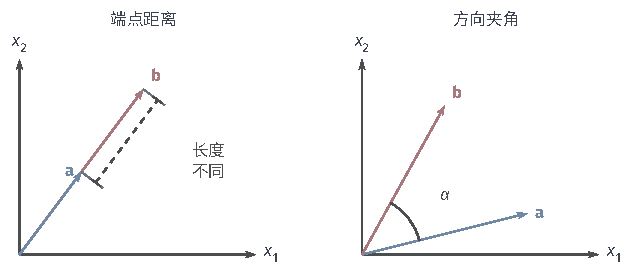
\includegraphics[width=107.322mm]{figures/06-foundations/01-basics/tikz/models-vector-comparison/figure.pdf}
  \caption{两种向量比较方式关注不同差异。左侧比较两个端点之间的距离，
  右侧比较向量方向之间的夹角。同向但长度不同的向量，余弦损失为零，欧氏误差仍大于零。}
  \label{fig:models-vector-comparison}
\end{figure}

数值误差是否符合任务中的相似性，还取决于所用表示。一张图像只平移一个像素，内容可能基本相同，许多对应像素却已有较大差异。位置必须精确对应的重构适合逐像素比较；关心物体内容的任务则可能先提取特征，再比较表示。选择度量时，我们也在选择要保留哪些差别。

\paragraph{概率分布的差异}
\label{sec:models-probability-objectives}

概率输出包含的信息多于最终类别或均值。邮件分类可能还要求概率能够用于风险判断，分布学习要描述样本出现的规律，模型模仿则可能要求两个模型对各类别给出相近概率。面对这些任务，只比较选出的答案会漏掉其余概率信息，我们需要评价分布本身。

有限类别的概率分布可以逐项比较。设目标$\bm{p}=(p_1,\ldots,p_k)^{\top}$、预测$\bm{q}=(q_1,\ldots,q_k)^{\top}$均非负且各自求和为一。模型给结果$j$的概率越低，$-\log q_j$越大；以目标概率$p_j$加权平均，便得到\term{交叉熵}（cross-entropy）：
\begin{equation}
  \operatorname{CE}(\bm{p},\bm{q})=-\sum_{j=1}^{k}p_j\log q_j.
  \label{eq:models-cross-entropy}
\end{equation}
其中$p_j=0$的项约定为零，$p_j>0$而$q_j=0$时取无穷大。已知样本类别为$c$时，可以把目标写成$p_c=1$、其余为零的\term{独热表示}（one-hot representation），损失于是化为$-\log q_c$。给正确类别$0.9$比$0.1$产生的损失小，而$q_c$趋近零时损失趋向无穷大，故自信的错误受到较重惩罚。本节使用自然对数（可参考\BookVolumeRef{vol:mathematical-preliminaries-lower}{卷2《数学准备：概率、因果与决策》}）。

预测分布与目标分布相同时，交叉熵仍可能为正，因为目标本身也可能有不确定性。若要把完全相同的分布记为零差异，就要从交叉熵中扣除目标自身不确定性贡献的那一项，得到\term{KL散度}（Kullback--Leibler divergence）：
\begin{equation}
  D_{\mathrm{KL}}(\bm{p}\Vert\bm{q})
  =\sum_{j=1}^{k}p_j\log\frac{p_j}{q_j}.
  \label{eq:models-kl}
\end{equation}
KL散度也沿用前面的零质量与零预测概率约定。把对数比值拆成$\log p_j-\log q_j$，求和即得$D_{\mathrm{KL}}(\bm{p}\Vert\bm{q})=\operatorname{CE}(\bm{p},\bm{q})-\operatorname{CE}(\bm{p},\bm{p})$，后一项正是目标自身的不确定性（熵）。散度非负，且仅在两个分布相同时为零；这一性质可由对数函数的凹性经Jensen不等式得到。目标固定时，$\operatorname{CE}(\bm{p},\bm{p})$不随预测改变，因此两种准则的最小化要求相同。交换目标与预测会改变加权所依据的分布，KL散度一般也会改变。

也可以把预测概率与观测类别的独热向量直接比较。类别为$c$时，$\bm{e}_c$仅第$c$项为1，\term{Brier评分}（Brier score）写为
\begin{equation}
  \ell_{\mathrm{Brier}}(\bm{q},c)
  =\sum_{j=1}^{k}(q_j-\mathbb{I}\{j=c\})^2.
  \label{eq:models-brier}
\end{equation}
按这个求和定义，评分在$0$到$2$之间：全部概率给正确类别时为$0$，全部给某个错误类别时为$1^2+1^2=2$。二分类若只用正类概率$q\in[0,1]$和标签$y\in\{0,1\}$计分，常写为$(q-y)^2$；上式同时计算两个类别的偏差，等于这个单项评分的两倍。

Brier评分为什么鼓励如实报告概率？设真实类别按分布$\bm{p}$随机出现，则指示量$\mathbb{I}\{j=c\}$的期望为$p_j$、方差为$p_j(1-p_j)$。对每一项取期望，有$\mathbb{E}(q_j-\mathbb{I}\{j=c\})^2=(q_j-p_j)^2+p_j(1-p_j)$，求和得到$\lVert\bm{q}-\bm{p}\rVert_2^2+\sum_j p_j(1-p_j)$。后一项与预测无关，前一项在$\bm{q}=\bm{p}$时为零，所以期望评分在预测等于真实分布时最小。与交叉熵相比，Brier评分对极端错误的惩罚有上限，交叉熵则没有，两者由此赋予少数自信错误不同权重。Brier评分既可训练也可评价概率预测，是较早提出的概率预报准则之一\scite{brier1950}。

以上准则都假定目标分布$\bm{p}$已知。学习数据分布时情况不同：我们只掌握从真实分布中抽出的样本，并不知道真实分布本身，无法直接计算交叉熵。替代做法是让模型密度$p_{\bm{\theta}}(\bm{x})$给已观测样本较大的密度，即最小化平均负对数似然：
\begin{equation}
  \ell_{\mathrm{NLL}}(\bm{\theta})
  =-\frac{1}{n}\sum_{i=1}^{n}\log p_{\bm{\theta}}(\bm{x}_i).
  \label{eq:models-negative-log-likelihood}
\end{equation}
它与第\ref{sec:models-probabilistic}小节的似然一致：最小化平均负对数似然，就是最大化样本的似然；GMM等分布模型可以使用这一目标。式中的平均只评价这$n$个样本。它与交叉熵的联系在于：若把样本平均改为按真实分布$P$取期望，就得到总体负对数似然，即“真实分布作目标、模型作预测”的交叉熵。严格地说，需要假设$P$和模型$Q_{\bm{\theta}}$相对共同参考测度有密度，$P\ll Q_{\bm{\theta}}$，且真实密度的对数在$P$下可积、模型负对数密度的期望有定义；在这些条件下，与离散情形一样，交叉熵等于$P$的（微分）熵加$D_{\mathrm{KL}}(P\|Q_{\bm{\theta}})$，固定$P$后最小化它等价于在模型类内减小KL散度。

这个等价关系说明了样本平均在“瞄准”什么，但没有保证达到它。模型失配时，即使求得类内最优解，它也只能近似真实分布；有限样本的经验优化还须控制整个候选模型族上经验目标与总体目标的差异以及求解误差，不能只凭独立同分布抽样推出总体最优。若$y$是有限类别标签，拟合$p_{\bm{\theta}}(y\mid\bm{x})$时，相应负对数似然就是分类交叉熵。

上述准则都逐个结果比较概率，并不自动知道两个类别或位置相距多远。若任务关心概率质量移动的距离，还需要把结果空间中的距离纳入准则。

\subsection{关系与结构准则}
\label{sec:models-spatial-objectives}

没有逐样本答案时，我们可以规定对象应当怎样组织；已有答案时，任务也可能在逐样本正确之外提出关系要求。聚类要求同组样本紧凑，检索要求相关样本更近，分类可以要求正确一侧的样本还离边界足够远，降维则限制表示所在空间的维数。这些关系与结构准则比较的对象各不相同；其中有些是必须满足的约束，有些是通过学习目标鼓励的性质。

\paragraph{样本到中心的距离}

K-means选择$k$个中心，让每个样本与最近中心的平方距离尽量小：
\begin{equation}
  \min_{\bm{\mu}_1,\ldots,\bm{\mu}_k}
  \frac{1}{n}\sum_{i=1}^{n}\min_{1\leq j\leq k}
  \lVert\bm{x}_i-\bm{\mu}_j\rVert_2^2.
  \label{eq:models-kmeans-objective}
\end{equation}
内层在固定中心下为样本选择归属，外层改变中心位置以缩小平均距离。簇编号来自这一几何准则，没有真实类别作参照。平方距离提高远点的影响，偏好围绕中心的紧凑群组。若换成$L_1$距离，固定分组后的最优中心为各坐标中位数，对少数远点通常更稳健；若方向更重要，则可另选基于余弦相似度的准则。

K-means的目标只直接缩小簇内平方距离，并未要求每两个簇都尽量远离。中心取各簇均值时，总平方离差可以分为簇内项与簇间项；固定数据后，前者减小会使后者增大。不过，簇间项衡量各中心相对总体均值的分散程度，不能保证所有簇对都充分分离。

\paragraph{样本到分类边界的间隔}

SVM在预测正确之外还鼓励留出\term{间隔}（margin）：硬间隔设定把正确一侧和余量写成约束；下面的合页损失则允许违反，但会惩罚错分或余量不足。令$y\in\{-1,+1\}$，得分$f(\bm{x})=\bm{w}^{\top}\bm{x}+b$，常用\term{合页损失}（hinge loss）为
\begin{equation}
  \ell_{\mathrm{hinge}}(y,f(\bm{x}))
  =\max\{0,1-yf(\bm{x})\}.
  \label{eq:models-hinge}
\end{equation}
乘积$yf(\bm{x})$把标签和得分合在一起：它为正表示分类正确，数值越大表示正确得越“有把握”。$yf(\bm{x})\ge1$时损失为零；落在$0$与$1$之间表示分对但余量不足，小于$0$表示分错，二者都按差额线性受罚。

只用合页损失还不够：把$\bm{w}$和$b$同乘一个大于一的数，所有得分同比放大，损失可以变小，边界$f(\bm{x})=0$的位置却没有变。真正有几何意义的是样本到边界的距离。当$\bm{w}\ne\bm{0}$时，样本到边界的有符号几何距离为$yf(\bm{x})/\|\bm{w}\|_2$；在得分余量固定为$1$的样本上，这个距离等于$1/\|\bm{w}\|_2$，权重范数越小，几何间隔越大。线性SVM因此在合页损失之外再惩罚$\|\bm{w}\|_2^2$，两项共同权衡余量违反与间隔大小。与K-means不同，它只关心边界附近的样本，不要求把全部同类样本压到一个中心附近。

\paragraph{相关样本之间的相对距离}

检索有时只需要保留相对次序：同一物体的两张照片应比不同物体的照片更近。令参照表示为$\bm{a}$、相关表示为$\bm{p}$、不相关表示为$\bm{n}$，指定距离$d$及余量$m>0$，\term{三元组损失}（triplet loss）比较两段距离：
\begin{equation}
  \ell_{\mathrm{triplet}}
  =\max\{0,d(\bm{a},\bm{p})-d(\bm{a},\bm{n})+m\}.
  \label{eq:models-triplet}
\end{equation}
相关样本至少近$m$时，损失为零，否则不足的差额计入损失。它规定相对关系，不要求表示围绕固定中心。效果依赖距离、样本配对和余量：容易满足的比较少有学习信号，错误配对会促成错误邻近关系。图\ref{fig:models-spatial-objectives}对照中心距离、分类间隔与相对距离；依据已知相似关系学习表示或距离，是\term{度量学习}（metric learning）的基本思路\scite{weinberger2009}。

\begin{figure*}[t]
  \centering
  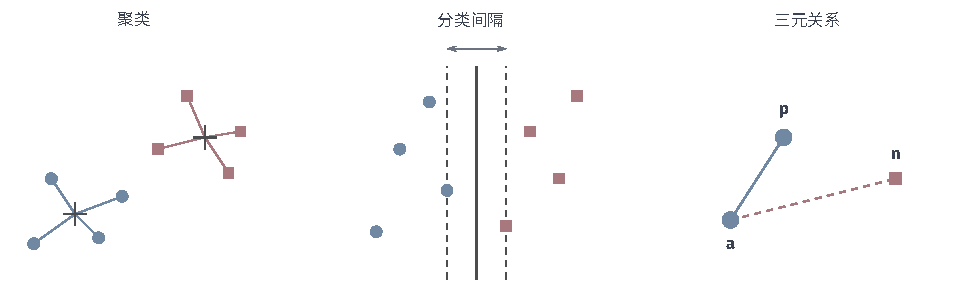
\includegraphics[width=161.406mm]{figures/06-foundations/01-basics/tikz/models-spatial-objectives/figure.pdf}
  \caption{三种几何要求。左侧缩短样本到所属中心的距离；中间让带标签样本与分类边界保持
  间隔；右侧要求相关样本比不相关样本更接近参照样本。三者分别比较不同的几何对象。}
  \label{fig:models-spatial-objectives}
\end{figure*}

\paragraph{低维结构}

PCA提出另一种组织要求：先把表示限制在低维空间，再减小重构误差。设保留$r<d$个方向，把它们作为列组成矩阵$\bm{U}\in\mathbb{R}^{d\times r}$，要求各列为单位长度且两两正交（$\bm{U}^{\top}\bm{U}=\bm{I}$）；记$\bar{\bm{x}}$为样本均值。样本中心化后投影到这些方向，得到$r$个坐标$\bm{U}^{\top}(\bm{x}_i-\bar{\bm{x}})$，再映射回原空间得到重构$\bar{\bm{x}}+\bm{U}\bm{U}^{\top}(\bm{x}_i-\bar{\bm{x}})$。PCA选择使平均重构误差最小的方向：
\[
  \min_{\bm{U}^{\top}\bm{U}=\bm{I}}\;
  \frac{1}{n}\sum_{i=1}^{n}
  \bigl\lVert(\bm{x}_i-\bar{\bm{x}})-\bm{U}\bm{U}^{\top}(\bm{x}_i-\bar{\bm{x}})\bigr\rVert_2^2.
\]
这里“低维”是硬约束，由$r$固定；误差是在约束内要尽量减小的量。

把四个例子放在一起看，中心距离保留紧凑群组，分类间隔保留边界余量，相对距离保留邻近次序，低维约束压缩表示。选用哪一种，取决于任务需要保留什么；一个模型也可以同时满足几种要求。

\subsection{轨迹与长期目标}
\label{sec:models-sequence-objectives}

前面的准则评价给定样本上的预测误差、样本间的关系或表示的重构与结构；它们还没有把行动造成的后续状态变化计入评价。当模型的输出是一个会改变环境的动作时，评价对象就变了。机器人导航中的一步不能只按眼前离终点多近评价：看似向前的动作可能进入死路，暂时绕行却可能更早到达；游戏决策和连续资源调度也由当前动作改变后续状态与奖励。此时要评价的是一整段行动，而不是某一步的即时得分。

\paragraph{长期目标与监督学习的区别}

与前面固定样本上的监督学习相比，由奖励驱动的行动学习在三处不同。

第一，答案的形式不同。监督目标给出与输入配对的答案；行动设定却不直接提供“这一状态下的正确动作”，只在动作之后陆续给出奖励。一个动作的好坏要等后续轨迹展开才能判断，把最终结果归功或归咎于之前哪些动作，称为信用分配问题。

第二，数据的来源不同。前面的分析把训练记录视为固定的独立样本，这里的动作却会改变下一步遇到的状态：今天选择探索未知区域，明天面对的数据分布就随之改变，学习到的动作规则影响它自己将来能看到什么。需要说明，监督学习也可以处理相关序列和在线反馈，独立性并不是区分两种范式的定义条件。

第三，评价的对象不同。监督学习以逐条预测损失为准则，这里要评价行动后果的累计与期望。动作规则（策略）与环境共同决定一条轨迹；常见目标先累计轨迹中的多步奖励，再对环境随机性和动作选择导致的各种可能轨迹取期望，也可以比较长期运行的单位时间平均回报。两者都无法由单步即时误差代替，短期奖励甚至可能与长期回报方向相反，例如先投入成本再获得收益。状态、动作、奖励、策略与这些目标的正式定义见第~\ref{sec:reinforcement-learning}节。

\paragraph{长期目标带来的额外困难}

期望回报还不能说明结果是否稳定：若失败概率也受到限制，目标之外就要加入相应约束；若轨迹很长或关键事件罕见，有限次交互对长期表现的估计会剧烈波动，探索未知动作与利用当前最优动作之间也必须作出权衡。长期目标内部仍可以使用熟悉的损失：价值模型预测未来累计回报，训练时可以用平方误差，但这个预测任务服务于决策目标。反过来，输出是序列也不意味着在优化长期目标——逐词预测文本在每个位置都有真实词可比较，其学习准则仍是逐位置的概率分布拟合，属于监督学习。

本节最后还要分清准则与算法两件事。学习目标规定怎样比较结果，可以由预测误差或累计回报等量构成；梯度下降、交替更新等算法规定怎样寻找更好的结果。准则也不一定作用于整个模型：决策树每一步评价候选分裂，未必优化整棵树的单一全局目标；近邻分类没有参数拟合目标，只在查询时按距离选出$k$个已保存样本投票。因此，列出准则以后，还要交代它作用于整个模型、某个步骤，还是对当前方法不适用。

\FloatBarrier
\section{模型维度的交叉与组合}
\label{sec:models-crossing}

前文多次遇到维度之间的交叉：非线性模型可以只有固定数量的参数，概率模型也可以只返回一个数。如果五个维度互相决定，我们只需记住少数几种典型模型；正因为它们可以独立变化，才需要逐项判断。本节先在同一个温度任务上每次只改变一项设定，看哪些性质随之改变、哪些保持不变；再用分类和聚类两张对照表检验这套描述；最后讨论多个模型怎样组合，以及怎样在方案之间作出选择。

\subsection{模型维度的组合}
\label{sec:models-dimension-combination}

以气象特征预测明日温度，先固定输入表示。我们可以选用固定数量的权重计算仿射函数，返回一个温度值，再以平方误差拟合数据。这个具体方案采用参数化表示、非概率语义和线性关系，接口返回标量，学习准则比较预测温度与观测值。任务名称只说明要预测什么，这些属性都由方案的具体设定确定。

若仍用仿射函数计算均值，却同时估计方差并指定高斯分布，固定维参数化方式得以保留，表示规模则因方差参数而增加。均值的关系形式也保留，但模型开始描述温度分布，训练准则相应转为评价观测数据的似然。

我们还可以保留点预测接口，改用含非线性激活的固定结构神经网络：参数化方式不变，关系形式改变；若让它计算分布参数，便又加入概率语义。近邻回归依赖随数据增加的实例，构成非参数化、非概率方案；高斯过程不受固定有限维系数限制，同时为可能函数与预测结果建立分布。这些例子说明，同一任务并不固定五个维度的取值。

各项设定也不能任意拼接，输出所含的信息必须在评价中得到对应的解释。标量温度可以用平方或绝对误差比较，类别概率可以用交叉熵或Brier评分评价；类别编号只是身份，编号相减不能表示误判代价；模型若同时报告方差，只看均值误差就会漏掉方差提供的信息。表示限制同样会进入准则：K-means用有限中心描述群组，就缩小样本到中心的距离；PCA限制低维子空间，就评价重构误差。五维分析的用处，正是检查表示规模、概率语义、关系形式、输出和评价依据能否共同完成任务。

\subsection{分类模型的五维比较}
\label{sec:models-classification-grid}

现在用分类检验这套描述。章首的权重、规则树和近邻都能预测类别，它们在哪些方面相近，又在哪些方面不同？表\ref{tab:models-classifiers}给出九个具体版本。沿列阅读可比较同一属性，沿行阅读则可检查一个模型的全部设定。

同一个方法名常常对应多个版本，各版本在五个维度上的取值可能不同，因此阅读表格前需要先限定其中几种版本。

高斯判别分析假设每类输入服从多元高斯分布，再用式\eqref{eq:models-generative-classification}计算后验。多元高斯由均值和\term{协方差}（covariance）矩阵确定，后者描述各方向的分散程度及特征之间的相关性。比较两类的对数后验之差时，各类高斯密度指数中的二次项$\bm{x}^{\top}\bm{\Sigma}^{-1}\bm{x}$在各类共用同一非奇异协方差矩阵$\bm{\Sigma}$时相互抵消，剩下输入的线性函数，边界因而是线性的；各类分别使用不同协方差时，二次项不再抵消，一般形成二次边界，这一版本称为\term{二次判别分析}（quadratic discriminant analysis）。

朴素贝叶斯取伯努利版本，以$0$、$1$记录词是否出现；当各类内特征概率严格位于零与一之间时，每个特征对对数几率的贡献只有“出现”和“不出现”两个取值，类别对数几率因而可写成二值特征的线性函数。神经分类器先对各类别得分取指数，再除以这些指数值的总和，得到非负且总和为一的类别概率，并以分类交叉熵训练。

硬标签决策树需要一个衡量“分得好不好”的标准。它用基尼不纯度$1-\sum_c\hat p_c^2$衡量一个节点内类别的混杂程度，其中$\hat p_c$是该节点中$c$类样本的比例：纯节点的不纯度为$0$，二分类样本各半时为$1-2\times0.5^2=1/2$。每个候选分裂按左右子节点的样本比例加权其不纯度，再与父节点比较；算法在满足预定深度、叶节点样本量等限制的候选中，逐步选择不纯度下降最大的分裂。这是局部贪心准则，每一步只看眼前最好的分裂，不保证所得整棵树全局最优。

\begin{table*}[htbp]
  \centering
  \footnotesize
  \setlength{\tabcolsep}{4pt}
  \renewcommand{\arraystretch}{1.25}
  \begin{tabularx}{\linewidth}{@{}>{\raggedright\arraybackslash}p{28mm}>{\raggedright\arraybackslash}p{20mm}>{\raggedright\arraybackslash}p{14mm}>{\raggedright\arraybackslash}p{22mm}>{\raggedright\arraybackslash}p{20mm}>{\raggedright\arraybackslash}X@{}}
    \toprule
    \textbf{具体模型设定} & \textbf{参数化方式} & \textbf{概率语义} & \textbf{关系形式} & \textbf{输出接口} & \textbf{学习目标} \\
    \midrule
    线性SVM & 参数化 & 非概率 & 线性得分 & 得分、类别 & 合页损失与权重惩罚 \\
    逻辑回归 & 参数化 & 概率 & 线性对数几率 & 类别概率 & 条件负对数似然，即分类交叉熵 \\
    高斯判别分析，共享协方差 & 参数化 & 概率 & 线性对数后验之差 & 类别概率 & 带标签数据的联合似然 \\
    伯努利朴素贝叶斯 & 参数化 & 概率 & 二值特征的线性对数几率 & 类别概率 & 带标签数据的联合似然，即类别比例与类内特征概率 \\
    高斯核SVM & 非参数化 & 非概率 & 非线性得分 & 得分、类别 & 特征空间中的间隔目标 \\
    二次判别分析 & 参数化 & 概率 & 一般为二次边界 & 类别概率 & 带标签数据的联合似然 \\
    固定结构、类别概率读出的非线性神经分类器 & 参数化 & 概率 & 非线性得分 & 类别概率 & 分类交叉熵 \\
    硬投票$k$近邻 & 非参数化 & 非概率 & 局部投票形成的分段规则 & 类别 & 无参数拟合目标；查询时按距离取$k$个邻居并硬投票 \\
    硬标签决策树，叶数可增长、按基尼不纯度分裂 & 非参数化 & 非概率 & 条件分支与分段规则 & 类别 & 逐步最大化基尼不纯度下降 \\
    \bottomrule
  \end{tabularx}
  \caption{分类模型的五维比较。表中采用所列的具体版本；概率模型均可进一步返回最大概率类别。
  “概率语义”按是否建立类别或联合分布判断，不能只由最终是否返回标签判断。}
  \label{tab:models-classifiers}
\end{table*}

与其逐行复述表格，不如固定一两个维度，看其余维度怎样变化。下面依次固定边界形状、考察表达能力的扩展方向、比较输出与准则。

先固定线性边界。线性SVM、逻辑回归、共享协方差的高斯判别分析和伯努利朴素贝叶斯，都可以用固定数量的参数得到线性得分或线性对数几率，但拟合的对象不同：SVM以间隔准则学习得分、不建立类别分布；逻辑回归直接拟合$p(y\mid\bm{x})$，不仅确定分界，还给出分界两侧的类别概率；后两者先拟合$p(y)p(\bm{x}\mid y)$再求后验。生成式路线因此还能利用所建联合分布采样或处理缺失观测，但也要为类内输入分布承担假设和估计代价。

哪条路线更省样本，不能只由名称判断。Ng与Jordan比较朴素贝叶斯和逻辑回归时发现，具体条件下两者可能在不同样本量区间各占优势：生成式方法可以较快接近它自身的极限错误率，而判别式方法在样本更多时可以接近更低的极限错误率\scite{ng2001}。这种“接近极限的速度”与“极限风险多低”是两个不同问题，不能合并为生成式模型普遍更好的结论。边界形状相同，也不意味着概率假设、估计目标和训练代价相同。

再看表达能力怎样扩展。从线性版本出发，不同模型选择了不同的扩展方向：SVM改用高斯核后保留间隔准则和得分输出，边界可以弯曲，表示规模却随支持向量数增长；高斯判别分析改用各类不同协方差得到二次边界，仍保持参数化概率建模；固定结构神经分类器与逻辑回归一样直接拟合条件分布并用交叉熵训练，中间层能形成比该逻辑回归更丰富、但仍受固定架构限制的得分关系，训练还需处理结构选择、调参与非凸优化；$k$近邻和叶数可增长的决策树直接让表示随数据扩张，不做全局参数拟合，代价取决于保留实例、分区规模和查询方式，局部预测在观测范围之外还缺少直接依据。因此，非线性能力的增加并不必然改变概率语义，也不保证偏差、方差和成本按同一方向变化。更丰富的表示可能减小近似误差，同时增加估计或求解负担；这些变化需要在相同任务、样本量和训练预算下比较。

最后比较输出接口与学习准则。SVM交得分、逻辑回归交概率、硬投票近邻和硬标签树只交类别：概率接口可以直接支持风险决策和拒绝判断，但必须检验校准，发现偏差时再按适用条件修正，名义概率不能直接当作真实频率；硬标签接口较简单，却不保留置信信息，可靠性仍须另行评价。准则也对应不同的优化承诺：SVM优化一个明确的全局凸目标，树按基尼不纯度逐步贪心分裂、不保证整棵树全局最优，近邻则没有这里所说的参数拟合目标，新输入的邻居检索与投票主要在查询时完成，但特征处理和检索索引可以事先计算。表中的“硬投票”“硬标签”只限定此次比较的版本——若改用近邻频率或叶节点类别比例，概率语义和接口都要重新说明；方法名称允许多个版本，具体设定才是比较的依据。

\subsection{聚类模型的五维比较}
\label{sec:models-clustering-grid}

取消邮件标签以后，我们要决定哪些邮件归在一起。分组可以依据同一中心附近的位置、同一潜在分布，或邻近样本形成的连通区域。除K-means和GMM外，表中还有四种组织方式。高斯核K-means在核特征空间中执行K-means，使原空间的分配边界可以弯曲。\term{模糊C均值}（fuzzy c-means）不强制每个样本只属于一组，而为它保留对各中心的隶属度，即属于各组的程度。\term{DBSCAN}（density-based spatial clustering of applications with noise）按半径邻域中的样本数识别稠密区域，从邻域足够稠密的核心点出发连接扩展群组。\term{凝聚层次聚类}（agglomerative hierarchical clustering）从每个样本自成一组开始逐步合并，保留一棵多层分组树；表中采用的\term{Ward方法}每次合并使簇内平方离差增加最少的一对簇。表\ref{tab:models-clusterers}据此汇总七个版本的分组依据、表示和输出。

\begin{table*}[htbp]
  \centering
  \footnotesize
  \setlength{\tabcolsep}{4pt}
  \renewcommand{\arraystretch}{1.25}
  \begin{tabularx}{\linewidth}{@{}>{\raggedright\arraybackslash}p{28mm}>{\raggedright\arraybackslash}p{20mm}>{\raggedright\arraybackslash}p{14mm}>{\raggedright\arraybackslash}p{22mm}>{\raggedright\arraybackslash}p{20mm}>{\raggedright\arraybackslash}X@{}}
    \toprule
    \textbf{具体模型设定} & \textbf{参数化方式} & \textbf{概率语义} & \textbf{关系形式} & \textbf{输出接口} & \textbf{学习目标} \\
    \midrule
    K-means & 参数化 & 非概率 & 线性两两分配边界 & 簇编号 & 样本到中心的平方距离 \\
    高斯核K-means & 非参数化 & 非概率 & 非线性分配边界 & 簇编号 & 核特征空间中的平方紧凑性 \\
    模糊C均值 & 参数化 & 非概率 & 隶属度非线性；硬分界线性 & 隶属度向量、编号 & 隶属度加权的簇内平方距离 \\
    GMM，共享协方差 & 参数化 & 概率 & 线性两两分配边界 & 组别概率、编号 & 观测数据的似然 \\
    GMM，不同协方差 & 参数化 & 概率 & 一般为二次分配边界 & 组别概率、编号 & 观测数据的似然 \\
    DBSCAN & 样本内邻域图随$n$增长 & 非概率 & 线性/非线性不适用；邻域连通关系 & 簇编号、噪声标记 & 邻域计数与连通规则，无统一的误差最小化目标 \\
    Ward层次聚类 & 含$n$个叶节点的样本内层次树 & 非概率 & 线性/非线性不适用；逐步合并的层次关系 & 层次树、截取后的簇编号 & 每步最小化簇内平方离差的增量 \\
    \bottomrule
  \end{tabularx}
  \caption{聚类方法的五维比较。参数化设定固定输入维数与中心或成分数。
  DBSCAN与Ward层次聚类主要组织已有的$n$个样本，第二列记录其邻域图或层次树怎样随样本数增长，
  而不把输出标签数量当作模型参数；二者也不直接对应可按线性或非线性归类的作用于新预测输入的函数。}
  \label{tab:models-clusterers}
\end{table*}

聚类没有预先给出的唯一分组答案，比较这些模型时要说明“用什么结构组织群组”。下面按三组问题对比。

先比较中心模型内部的几种变化。K-means只用$k$个中心和平方距离，计算快、结果易解释，但它倾向于找出大小相近、近似球形的群组：两中心之间的分配边界是线性的，见式\eqref{eq:models-kmeans-boundary}。高斯核K-means保留中心与紧凑性准则，在核特征空间比较样本与原型，原空间边界可以弯曲、原型随样本表示，代价是表示规模增长和核参数选择\scite{dhillon2004}。模糊C均值不改变中心模型，只把硬分配换成隶属度：交界处样本可以部分属于多组，但隶属度虽总和为一，却不是从观测分布推出的后验概率，它换来的是软性输出而非概率解释\scite{bezdek1984}。

再比较几何紧凑性与概率建模。GMM用混合比例和多个高斯成分描述联合分布、以似然学习参数，用后验表示组别概率；共享协方差时二次项抵消、边界线性，协方差不同时保留二次边界。与K-means相比，它能描述群组的大小、形状和重叠、给出归属不确定性，但必须付出高斯形状假设、更多参数和似然估计（含局部最优）的代价。这对应第\ref{sec:models-probability}节的结论：同样一条两两边界，几何方法用距离解释分组，概率方法用分布和后验解释分组。

最后比较全局固定结构与局部、层次结构。DBSCAN不预设中心或成分，把无法归入任何稠密区域的点明确标为噪声：它能发现任意形状的群组、天然处理离群点，却只组织已有的$n$个样本，规模随$n$增长，给新样本分配还要另定冲突与拒绝规则\scite{ester1996}。Ward层次聚类所得的树以$n$个样本为叶、可在任意层级截取，提供多粒度分组，代价是树的存储、合并的贪心不可逆和新样本插入困难\scite{ward1963}。因此，即使所有方法最终都输出簇编号，它们保留的信息也不同：中心模型给可复用的原型，概率模型给可检验的归属不确定性，密度方法给局部形状和噪声标记，层次方法给分组的多个粒度——选型时要先问任务真正需要哪一种群组信息。

\subsection{模型组合与选择}
\label{sec:models-combination-selection}

实际系统还可把多个模块连接起来。PCA之后使用K-means，是先压缩表示再分组；神经网络之后接线性分类器，是先形成非线性特征再计算线性得分。对后一个系统，最后一层线性并不意味着整体对原输入线性。描述组合时，需要逐个检查模块，也要说明它们传递什么结果。

模块的连接方式还涉及怎样训练。分阶段方案先学习上游表示，再固定它训练下游模型；端到端方案按最终目标共同调整相关参数。上游目标是否保留了下游所需的信息，需要专门检查：压缩器可能重构得很好，却删除了分类所依赖的微小差别。

多个模型也可以对同一个输入共同预测，称为\term{集成学习}（ensemble learning）。分类随机森林可让多棵有差异的树分别预测，再按多数投票或类别概率平均得到最终类别；梯度提升则逐步拟合当前目标中的修正量，并把各项加到已有预测上。后一过程旨在降低所用训练目标，不保证新样本表现随每次加入而改善。说明这样的系统时，既要交代基模型怎样产生差异，也要写清各输出怎样合成最终结果。

五维描述明确了模型假设，却还不能决定哪种方案在当前任务中更好。我们需要先按任务约定评价指标及其优劣方向，在相同的验证样本与可用信息条件下比较，再结合数据需求、存储与查询成本、解释需求，以及分布变化下的可靠性作出选择。

\section{本章小结}
\label{sec:models-summary}

本章开头问：权重、规则树和近邻可能给出相同的标签，比较它们时应该考察什么？回答分两层。第一层分清模型族、学习规则与训练模型：候选模型类限定允许的关系，学习规则利用训练样本作出选择，所得参数或保存的实例确定训练模型。第二层是五个比较维度：参数化方式说明表示受到的限制，概率语义说明是否用分布描述变量，关系形式说明变量怎样联系，输出接口说明交付的结果及其含义，学习目标把任务评价接到候选模型上，可以比较逐样本答案、对象之间的关系或整段轨迹。

回到章首的三种办法：逻辑回归保存固定数目的权重，用线性对数几率给出类别概率，按交叉熵选择参数；叶数可增长的决策树随数据增加分支，以条件规则划分区域，按不纯度逐步分裂；kNN保存全部实例，在查询时按距离投票，没有参数拟合目标。三者给出同一个标签时，这些差别仍决定了它们需要多少数据和存储、能否报告置信程度，以及在数据变化时怎样表现。

五项要分别判断，因为它们会交叉：线性与非线性计算都可以用于概率预测，固定参数也可以确定分布，类别编号和簇编号形状相同、评价依据却不同。五项又要互相配合，因为输出所含的信息必须在评价中得到解释，表示限制也会进入学习准则。学习准则属于完整学习设定，不是表示本身的属性；没有显式拟合目标的方法，要说明这一例外及其实际使用的规则。

\paragraph{扩展阅读}

下一章先转向经验与反馈：第\ref{chap:machine-learning-paradigms}章会说明它们改变时，学习怎样组织。第\ref{part:learning-theory}部分再在明确条件下研究算法能否从有限经验获得低风险结果，第\ref{part:trustworthy-ml}部分检查应用中的环境、群体、权限与风险要求。进一步阅读可从\BookVolumeRef{vol:classic-models}{卷4《模型：经典模型》}和\BookVolumeRef{vol:neural-network-models}{卷5《模型：神经网络模型》}进入相应模型专题。
